\section{Second-Order Accurate Base Schemes}\label{sec:basefv}
We are interested in solving hyperbolic conservation laws 
\begin{equation}
\begin{aligned} \label{eq:conslaw2D}
\frac{\partial}{\partial t}	\mathbf{u} + \nabla \cdot
\mathbfcal{F}(\mathbf{u})  = \mathbf{0}
\end{aligned}
\end{equation}
on the domain $\Omega \subset \mathbb{R}^2$ where $\mathbf{u}(x,y,t) \in \Omega \times [0,T]$ is a vector of conserved quantities, $T$ is the final time, and $\mathbfcal{F} = [\mathbf{F}, \mathbf{G}]$ is the flux function.  We discretize $\Omega$ into a cut cell mesh of cells $\Omega_{i,j}$.  A typical cut cell mesh, called the base grid, is given in Figure \ref{fig:2dfig}.  On the domain interior, $\Omega_{i,j}$ are Cartesian cells (quadrilaterals) of size $\Delta x$ in the $x$ direction and $\Delta y$ in the $y$ direction.  On the domain boundary there is a border of irregular polygonal cells, called cut cells.  
A line segment is used in each cut cell to represent
the intersection with the geometry.
We use cell-centered discretizations in this work.



There are two issues when applying an explicit finite volume scheme to a cut cell
mesh.  For accuracy, the scheme needs to be modified in the cut cells. Second, 
the scheme needs to be stabilized in the cut cells if using a fixed timestep $\Delta t$ 
based on the full cells. In the $h$-box method these two concerns were addressed
simultaneously, but in general they aren't.

We will use two very different second order discretizations of \eqref{eq:conslaw2D}: the method of lines
(MOL) approach and the MUSCL scheme.
These fully discrete finite volume methods, described in Section \ref{sec:mol} and \ref{sec:muscl},
are referred to as the base schemes.  Both schemes require linear 
reconstruction on grid cells,
outlined in Section \ref{sec:limit}.  
%The high-order extension of MOL and SRD  will be described in Appendix \ref{sec:ho}. 
Finally, both second order schemes evaluate the flux at
the boundary in the examples of Section \ref{sec:compResults} by extrapolating the
pressure to the boundary midpoint. 
We do not discuss domain boundary conditions in this paper,  since 
these procedures are  standard, and do not change due to cut cells.

\begin{figure}
\begin{center}
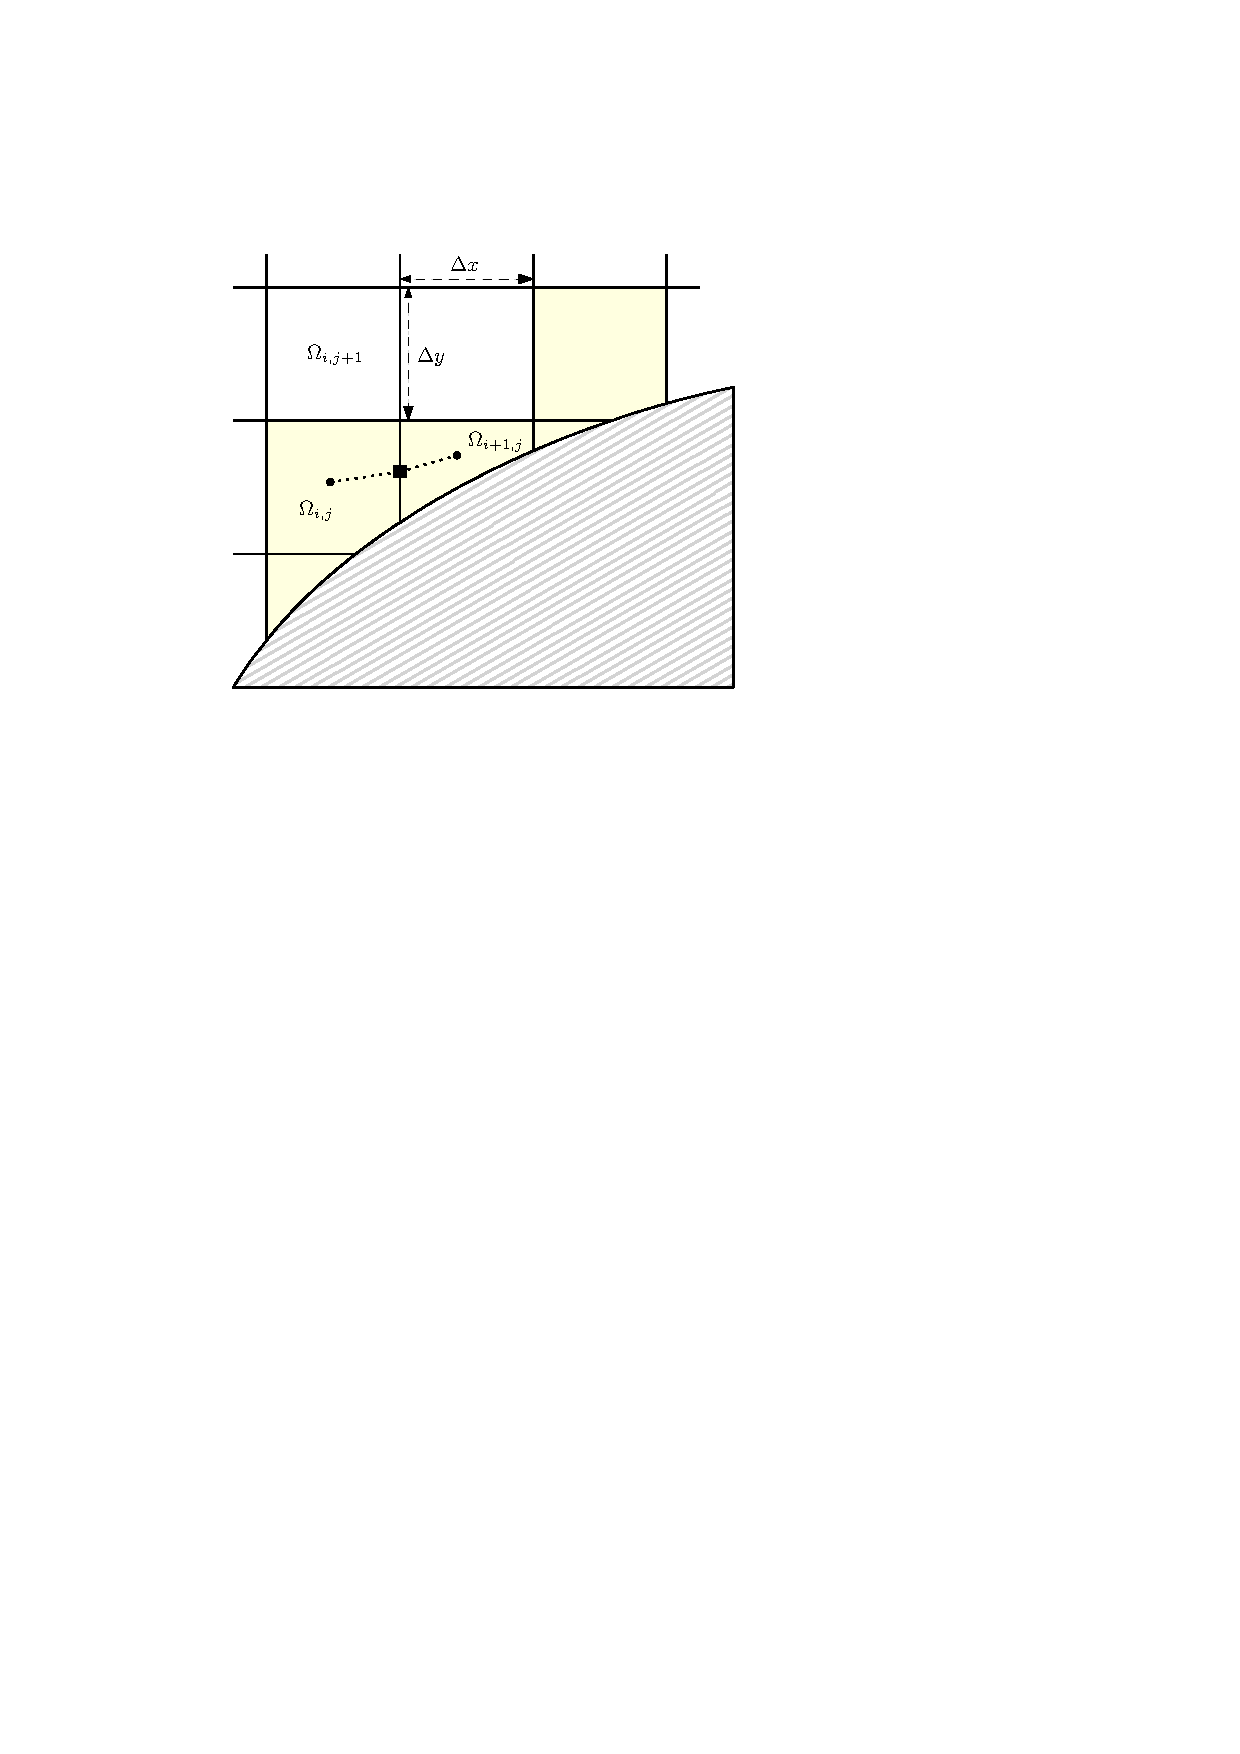
\includegraphics[width=3.0in]{figs/example_ccmesh.pdf}
\caption{\sf Example base grid in two space dimensions. The cells shaded
in yellow are the cut cells.  Both the method of lines (Section
\ref{sec:mol}) and MUSCL (Section \ref{sec:muscl}) schemes require
gradient information to reconstruct to the edge midpoint, indicated with
a square $(\blacksquare)$.} 
\label{fig:2dfig}
\end{center}
\end{figure}


\subsection{Method of lines} \label{sec:mol}

After generating the cut cell mesh, we approximate the solution to \eqref{eq:conslaw2D} on the base grid using a finite volume method of the form
\begin{equation}\label{eq:fvscheme}
\frac{d}{dt}\mathbf{U}_{i,j} =- \frac{1}{V_{i,j}} \int_{\partial \Omega_{i,j}} \mathbfcal{F} ^* \cdot \mathbf{n} ~dl,
\end{equation}
where $\mathbf{U}_{i,j}$ is a vector of the cell averages on $\Omega_{i,j}$, $\partial \Omega_{i,j}$ is the cell boundary, $\mathbf{n}$ is an outward facing normal, and $\mathbfcal{F}^*$ is a numerical flux function.

Second order accuracy in space is achieved by reconstructing a gradient on each
cell and using it to evaluate the numerical flux at the face midpoints,
illustrated in Figure \ref{fig:2dfig}.  
In our numerical experiments, we use the local Lax-Friedrichs numerical 
flux to solve the Riemann problem at cell interfaces. The integral in \eqref{eq:fvscheme} is  approximated using the midpoint rule.

Second order accuracy in time is obtained by integrating \eqref{eq:fvscheme} using Heun's method.  This is a two-stage Runge Kutta method that can be written
\begin{equation}\label{eq:molscheme}
\begin{aligned}
	\mathbf{U}^{(1)} &= \mathbf{U}^{n} + \Delta t L(\mathbf{U}^n), \\
	\mathbf{U}^{(2)} &= \mathbf{U}^{(1)} + \Delta t L(\mathbf{U}^{(1)}), \\
	\mathbf{U}^{n+1} &= \frac{1}{2}( \mathbf{U}^{n} + \mathbf{U}^{(2)} ) ,	
\end{aligned}
\end{equation}
where $\mathbf{U}^{n}$ is the vector of solution averages on the entire cut cell mesh at time $t^n$,
$\mathbf{U}^{(1)}$,$\mathbf{U}^{(2)}$, are intermediate stages, and $L$ is the operator that results
from discretizing the right-hand-side of \eqref{eq:fvscheme}.
We derive the maximum stable time step on the base grid by using \eqref{eq:molscheme} to solve the linear advection equation on a Cartesian grid with advection velocity $(a,b)$.
Numerical evaluation of the amplification factor that results from a linear stability analysis reveals that a stable time step satisfies
\begin{equation}\label{eq:vn1}
\Delta t   \left( \frac{|a|}{\Delta x} + \frac{|b|}{\Delta y} \right)\leq 1.
\end{equation}
%We have verified \eqref{eq:vn1} by numerical evaluation of the amplification factor that results from a linear stability analysis.
For a discrete maximum principle to be satisfied, a tighter 
time step restriction 
\begin{equation}
\Delta t  \left( \frac{2\Delta x + 2 \Delta y}{\Delta x \Delta y} \right) \sqrt{a^2 + b^2}\leq 1 .
\end{equation}
is required \cite{giuliani2018analysis}, in addition to a limiter to prevent new extrema.
For the Euler equations, the advective speeds $a$ and $b$ are replaced
by the largest magnitude $x$ and $y$ velocities  plus sound speed.

For this method, we apply SRD stabilization to the stage updates
$U^{(1)}$ and $U^{(2)}$ in \eqref{eq:molscheme}, before they are added to 
form $U^{n+1}$.  This is needed since the tiniest cut cells may have
non-physical quantities that need to be stabilized before  the
next stage.  For example, the first step in approximating the Euler
equations is to convert the conserved variables to primitives variables.
This would break down for negative densities. SRD however does not break
down and conservatively and accurately adjusts these values.

\subsection{MUSCL scheme} \label{sec:muscl}
The MUSCL scheme is a one step method that is second order accurate in
space and time. A series of MUSCL schemes  was originated by van Leer 
\cite{vanleer:muscl}. The version we use\footnote{Thanks to Phil 
Colella for the original Cartesian mesh code and Riemann solver,  and for helpful discussions on the shear
layer instability and artificial viscosity.}
is due to Colella \cite{Colella:Unsplit}.
The method is briefly sketched here so that we can describe how it was
adapted for cut cells. 

On a regular cell $(i,j)$ the interface values on the 
faces are computed at the half-step in time $t^{n+1/2}$, and the left and right states
are passed to a Riemann
solver to compute the fluxes.
Using a Taylor series in space and time to second order,
and using the conservation law \eqref{eq:conslaw2D}  to replace the derivative in time, gives the value for the right cell
interface $(i+1/2,j)$ 
%& = \mathbf{U}_{i,j}^n + 
%\frac{\Delta t}{2} \frac{\partial \mathbf{U}_{i,j}^n}{\partial t} + 
%\frac{\Delta x}{2} \frac{\partial \mathbf{U}_{i,j}^n}{\partial x} \\[.08in]
%&  = \mathbf{U}_{i,j}^n + \frac{\Delta t}{2} 
%\left(-\frac{\partial \mathbf{F}_{i,j}^n}{\partial x} -
%\frac{\partial \mathbf{G}_{i,j}^n}{\partial y} \right)  +
%\frac{\Delta x}{2} \, \frac{\partial \mathbf{U}_{i,j}^n}{\partial x} \\[.08in]
%&
\begin{subequations}
\begin{align}
\label{eqn:taylor}
\mathbf{U}_{i+1/2,j}^{n+1/2}    
              &= \mathbf{U}_{i,j}^n +  
\frac{\Delta t}{2} \frac{\partial \mathbf{U}_{i,j}^n}{\partial t} + 
\frac{\Delta x}{2} \frac{\partial \mathbf{U}_{i,j}^n}{\partial x} \\[.08in]
              &= \mathbf{U}_{i,j}^n - \frac{\Delta t}{2} \, 
             \frac{\partial \mathbf{G}_{i,j}^n}{\partial y}  -
            \left( \frac{\Delta t}{2} 
            \frac{\partial \mathbf{F}_{i,j}^n}{\partial \mathbf{U}^n_{i,j}} -
             \frac{\Delta x}{2} \right) \,\frac{\partial \mathbf{U}_{i,j}^n}{\partial x}, 
\end{align}
\end{subequations}
The values at the other interfaces of full cells are similarly defined.


In the original method,
Riemann problems are solved in the transverse direction, e.g. between
centroids $(i,j)$ and $(i,j-1)$, at the edge $j-1/2$, to produce
$\mathbf{G}_{i,j-1/2}$. 
The terms were then differenced to compute 
\begin{equation}
\partial \mathbf{G}_{i,j}/\partial y =  (\mathbf{G}_{i,j+1/2} - \mathbf{G}_{i,j-1/2})/\Delta y .
\label{eqn:transdiff}
\end{equation}
On a uniform mesh 
the first order accurate errors in computing \eqref{eqn:transdiff} 
cancel, and the term itself is 
multiplied by $\Delta t$ in \eqref{eqn:taylor}.
For more details the reader is referred to \cite{Colella:Unsplit}.

At the cut cells the above procedure is no longer accurate,
since  the centroid values are not coordinate aligned near
the cut cells.
We make two modifications to the
computation of $\partial \mathbf{G}/\partial y$, known as the
transverse derivative since it is in the vertical direction
when computing the flux $\mathbf{F}$ in the horizontal direction.
First,
the solution is reconstructed in the transverse direction
to the edge midpoint so it is properly centered in cells that
are adjacent to a cut cell.  This is the situation
in Figure \ref{fig:2dfig} for cell $(i,j+1)$, for example.

Second, many cut cells will not have both edges in the
transverse ($y$) direction. Instead, for all cut cells we
instead compute
$ \partial \mathbf{G}_{i,j}^n / \partial y = ( \partial \mathbf{G}_{i,j}^n / \partial \mathbf{U}_{i,j}^n)( \partial \mathbf{U}_{i,j}^n / \partial y)$,
like the horizontal fluxes in \eqref{eqn:taylor}. This is linearly exact in the cut cells, 
if the gradients themselves are.
We also experimented with dropping this term in the cut cells
altogether. There was no stability problem with this, but it
does introduce an unnecessary difference from
the interior scheme, and would not be linearly exact.

\textit{Note:} it is the transverse derivative term that provides the so-called corner 
coupling, i.e. inclusion
of corner cells in the stencil. This is what  gives  the MUSCL scheme a linear stability limit of
\begin{equation}
\label{eqn:bigcfllimit}
\Delta t \, \max \left (\frac{|a|}{\Delta x} , \frac{|b|}{\Delta y} \right) \leq 1,
\end{equation}
where $(a,b)$ is the advection velocity.  

The trickiest term to adapt to cut cells was an artificial viscosity in the original method that was 
added to each flux, with a
coefficient proportional to the negative divergence of the flow.  The original
code used a large stencil to compute this divergence. We instead use a centered
difference to compute $u_x$ and $v_y$, and where possible, and  
take the max of this over a $3 \times  3$
neighborhood centered around each cell, so that cut cells get this dissipation too. 

\commentout{
As remarked above, it is the transverse derivatives that allows for the larger time
step given in \eqref{eqn:bigcfllimit}.
However, in the neighborhood of a shock the derivatives will be limited, and
possibly set to zero.
If these terms were not used  in the volume mesh, the time step would be reduced to 
\begin{equation}
\Delta t \, \left (\frac{u+c}{\Delta x} + \frac{v+c}{\Delta y} \right) < 1
\end{equation}
which could be as small as half the larger limit in eq. \eqref{eqn:bigcfllimit}.
However, as shown in \cite{mjb:stability2} for one space dimension, 
boundary cells can have
a local {\em cfl} number that is up to twice the stable {\em cfl} of the regular
mesh and the overall scheme remains stable.  We have not found any stability
problems due to limiting of this term.  
}

The multi-dimensional MUSCL scheme due to Colella has several additional
features to robustly handle strong shocks, such as not including terms in
predicting the interface state from characteristics that propagate 
away from the interface. These
steps do not change at the cut cells, so are not discussed here.  

Since MUSCL is a one-step scheme, the SRD stabilization is applied directly
before the final update
$\mathbf{U}^{n+1} = SRD(\mathbf{U}^{n} + \Delta t
L(\mathbf{U}^{n}))$, where $L$ is now the MUSCL operator.



\subsection{Gradient reconstruction and limiting }\label{sec:limit}

The computation of gradients, and for problems with discontinuities limiting
those gradients, arises independently of the finite volume scheme used. 
On the domain interior, when the stencil is regular and does not contain cut cells, standard schemes can be used.
In all our examples we use monotonized central (MC) differencing in both $x$ and $y$ directions.  The MC limited slope in the $x$ direction is
\begin{equation}
\sigma^n_{x,i,j} =  \begin{cases} 
\min \left ( \,  \lvert{ D_c}\rvert,\,
2 \lvert {D_+}\rvert,\,
2 \lvert{D_-}\rvert \,  \right ) \,\times 
\text{ sign } D_c, \quad \text{if} \;\;  D_+ D_- >  0,\\
0 \hspace*{2.8in} \text{otherwise}.
\end{cases}
\end{equation}
Here we use the standard differencing notation
$D_c = (U^n_{i+1,j}-U^n_{i-1,j})/(2 \, \Delta x)$ for the second order accurate central difference and
$D_+ = (U^n_{i+1,j}-U^n_{i,j})/\Delta x$,
$D_- = (U^n_{i,j}-U^n_{i-1,j})/\Delta x$ for the one-sided differences.  The MC limited slope in the $y$ direction is similarly defined.

For cut cells 
%and their neighboring full cells, 
we use a least squares gradient reconstruction algorithm, a standard procedure
for unstructured meshes.
%Cells that are two away from a cut cell can use any limiter with a five point stencil. 
A linear reconstruction of the solution on these cells is of the form
\begin{equation}
u^n_{i,j}(x,y) = U_{i,j}^n + \sigma^n_{x,i,j} \,(x-x_{i,j}) +
                     \sigma^n_{y,i,j}\,(y-y_{i,j}),
\label{eqn:lls}
\end{equation}
where $(i,j)$ is the index of either a cut cell or cell with an
irregular stencil, $(\sigma^n_{x},\sigma^n_{y})_{i,j}$ and $(x,y)_{i,j}$
are its gradient and cell centroid, respectively. The least squares
procedure finds the gradient that minimizes the $L_2$ residual when
evaluating  $u^n_{i,j}(x,y)$ at  neighboring cell centroids. 

In this work, we consider both first and second order accurate 
gradients.  The reconstructed first order gradient satisfies in the 
least squares sense
\begin{equation}\label{eqn:linrecon_base}
\sigma^n_{x,i,j}(x_{r,s} - x_{i,j}) +
\sigma^n_{y,i,j}(y_{r,s} - y_{i,j})=
U^n_{r,s} - U^n_{i, j} \quad \forall (r,s) \in R_{i,j},
\end{equation}
where $R_{i,j}$ is the set of cell indices used for slope reconstruction on cell $(i,j)$ in the 
base scheme.  Here, $R_{i,j}$ is the $3\times 3$ neighborhood  centered on $(i,j)$.
The reconstructed second order gradient satisfies in the least squares sense
\begin{equation}
\begin{aligned}\label{eqn:linrecon_base2}
&\sigma^n_{x,i,j}(x_{r,s} - x_{i,j}) +
\sigma^n_{y,i,j}(y_{r,s} - y_{i,j})  + \\
&\quad \frac{1}{2}\sigma^n_{xx,i,j}[(x_{r,s} - x_{i,j})^2 - S_{xx,i,j}]  + \\
& \quad \; \sigma^n_{xy,i,j}[(x_{r,s} - x_{i,j})(y_{r,s} - y_{i,j})-S_{xy,i,j}] +\\
&\quad  \frac{1}{2}\sigma^n_{yy,i,j}[(y_{r,s} - y_{i,j})^2 - S_{yy,i,j}]
 \; = \;  U^n_{r,s} - U^n_{i, j} \quad \forall (r,s) \in R_{i,j},
\end{aligned}
\end{equation}
where $\sigma^n_{xx,i,j}$, $\sigma^n_{xy,i,j}$, $\sigma^n_{yy,i,j}$ 
are quadratic degrees of freedom and are discarded.  In this case, $R_{i,j}$ is either the $3\times 3$ tile centered on $(i,j)$ when $(i,j)$ is a whole cell neighboring a cut cell, or the $5\times 5$ tile centered on $(i,j)$ when $(i,j)$ is a cut cell.
Note that a cut cell needs a larger neighborhood because 
approximately half of its cells are not in the flow domain.  

Regular cells that are adjacent to a cut cell will also need special treatment to
compute a second order accurate gradient. We have experimented with three  approaches
and found almost indistinguishable results. The simplest is to use the 
procedure mentioned above for cut cells
- fit a least squares polynomial in the $3 \times 3$ neighborhood centered on that cell.
We also tried $5 \times 5$ neighborhoods, in hope of smoother transitions between cut cells
and the interior cells.  Finally, we tried using a centered
gradient in only one dimension, if there was one, and using a recentering approach to 
compute the second order accurate difference in the other direction.  This has an overall
smaller stencil, but still uses the $3 \times 3$ neighborhood
if there is no regular direction,
and involves more testing.  

For problems with discontinuities, the gradient will need to be limited
to prevent overshoots and retain positivity for quantities like density and
pressure.
We use the Barth Jespersen (BJ)  limiter \cite{barth-jespersen} to limit on 
cut cell grids. 
This is a scalar limiter, where both $\sigma^n_{x,i,j}$ and $\sigma^n_{y,i,j}$ 
are reduced by the same scalar to prevent new extrema.  
We compute the minimum and maximum values over the reconstruction 
stencil $R_{i,j}$, 
\begin{equation} 
m_{i,j} = \max_{(r,s) \in R_{i,j}} U^n_{r,s} \text{ and } 
M_{i,j} = \max_{(r,s) \in R_{i,j}} U^n_{r,s}.
\label{eqn:bj1}
\end{equation}
The reconstructed gradient on cell $(i,j)$ is limited by a non-negative 
scalar $\alpha \in [0,1]$, so that when ${u}_{i,j}(x,y)$ 
is evaluated at the centroids of the neighborhoods in $R_{i,j}$ it
lies between $m_{i,j}$ and $M_{i,j}$.
(Apologies for reusing the symbol $\alpha$, since it is commonly 
used to describe Barth-Jespersen-type limiters, as well as the 
mesh width $\alpha h$  of small cells).

The limited numerical solution is
\begin{equation}
     \tilde{u}^n_{i,j}(x,y) = U_{i,j}^n + \alpha \, [{\sigma}^n_{x,i,j} ( x -  x_{i,j}) \, 
   + {\sigma}^n_{y,i,j}( y -  y_{i,j})].
\end{equation}
Define
\begin{equation}\label{eq:bj_alpha}
    \alpha_{r,s} = \begin{cases}
           \min \left(1,\frac{M_{i,j}-U_{i,j}^n}{U^n_{r,s} - U_{i,j}^n} \right)
    \quad  \text{ if } \,   U_{r,s}^n - U_{i,j}^n >  0,\\[.08in]
            \min \left(1, \frac{m_{i,j}-U_{i,j}^n}{U^n_{r,s} - U_{i,j}^n} \right)  
    \quad  \text{ if }  \, U^n_{r,s} - U_{i,j}^n < 0.\\[.08in]
             1    \hspace*{1.45in}  \text{if} \; \, U^n_{r,s} - U_{i,j}^n = 0.
    \end{cases}
\end{equation}
Then choose
\begin{equation}\label{eqn:alpha}
\alpha = \min_{(r,s) \in R_{i,j}} \alpha_{r,s} .
\end{equation}

By reconstructing to the neighboring cell centroids, this procedure is linearity preserving.  

The approach described above differs slightly from the original Barth-Jespersen limiter in
\cite{barth-jespersen}, where the numerical solution is reconstructed to 
points on cell interfaces.
This is often the procedure used on unstructured meshes. However cut cell meshes are much more
irregular and without this fix BJ can lead to much less accurate solutions.

